\renewcommand{\theequation}{\theenumi}
\renewcommand{\thefigure}{\theenumi}
\begin{enumerate}[label=\thesubsection.\arabic*.,ref=\thesubsection.\theenumi]
\numberwithin{equation}{enumi}
\numberwithin{figure}{enumi}

\item Find the distance between the following pair of points (2,3) and (5,7). 
\\
\solution
\input{solutions/1/1/Assignment_2.tex}

\item Find the areas of the triangles the coordinates of
    whose angular points are respectively: 
\begin{equation}
\Vec{P} =\myvec{5 \\2 }, \Vec{Q} =\myvec{- 9\\ -3 }\text{ and } \Vec{R} =\myvec{-3 \\-5}\\
\end{equation}
%
\begin{align} \label{2/2/3eq1}
\Vec{Q-P} & =\myvec{-9 \\-3 \\} -\myvec{5 \\2}\\
 & = \myvec{-14 \\ -5}
 \label{2/2/3eq2}
\Vec{R-P} & =\myvec{-3 \\-5 } -\myvec{5 \\2}\\
 & = \myvec{-8 \\ -7}
\end{align}


%     As the vector cross product of two vectors can also be expressed as the product of a skew-symmetric matrix and a vector.

% \begin{align} \label{2/2/3eq4}
%     \Vec{A}\times  \Vec{B}  = 
%     \myvec{
%     0&-a_{3}&a_{2}\\
%     a_{3}&0&-a_{1}\\
%     -a_{2}&a_{1}&0\\
%     }
%     \times \myvec{
%     b_{1}\\
%     b_{2}\\
%     b_{3}\\}
% \end{align}

%     Substituting values from equation \ref{2/2/3eq1} and \ref{2/2/3eq2} in above equation \ref{2/2/3eq4}, we'll get:
\begin{align} 
%\label{2/2/3eq5}
\because (\Vec{Q-P})\times ( \Vec{R-P} ) & = \myvec{0&0&-5\\0&0&14\\5&-14&0\\} \times \myvec{-8\\-7\\0\\}\\
 & = \myvec{0\\0\\58\\}
%\label{2/2/3eq5}
\implies \norm{(\Vec{Q-P})\times ( \Vec{R-P} )} =\sqrt{0^2 + 0^2+ 58^2} = 58,
\end{align}
area of the triangle is given by 
\begin{align} 
%\label{2/2/3eq3}
 \frac{1}{2}\norm{ (\Vec{Q-P})\times ( \Vec{R-P} )} = \frac{1}{2}(58) =29 
 \end{align}


% Substituting value from equation \ref{2/2/3eq5} in equation \ref{2/2/3eq3}, we'll get area of triangle:

% $\implies  units^2$



\item The coordinates of the vertices of a triangle are $(x_1,y_1)$, $(x_2,y_2)$ and $(x_3,y_3)$. The line joining the first two is divided in the ratio $l:k$, and the line joining his point of division to the opposite angular point is then divided in the ratio  $m:k+l$. Find the coordinates of the latter point of section. 
%
\\
\solution
From elementary analysis of coordinate geometry and in view of Fig.\ref{eq:solutions/2/22/f2}, as $\bf{D}$ divides the line AB in the ratio $AD:DC=l:k$, we have:

\begin{equation}
 {\bf{D}}=\frac{l{\bf{B}}+k\bf{A}}{l+k}
    \label{eq:solutions/2/22/eq4}
\end{equation}
The position vector $\bf{E}$ which  divides CD in the ratio $DE:EC=m:l+k$,  is clearly obtained by setting $l=m,k=l+k,\bf{A=D,B=C}$ and is given by: 

\begin{equation}
 {\bf{E}}=\frac{m{\bf{C}}+(l+k)\bf{D}}{m+l+k}
    \label{eq:solutions/2/22/eq5}
\end{equation}
 
Using Eq.\ref{eq:solutions/2/22/eq4} into Eq.\ref{eq:solutions/2/22/eq5} and simplifying yields :
\begin{equation}
 {\bf{E}}=\frac{m {\bf{C}}+l{\bf{B}}+k{\bf{A}}}{m+l+k}
    \label{eq:solutions/2/22/eq6}
\end{equation}

Where,
%\begin{align}
 $  \bf{A}  = \begin{pmatrix}
           x_{1} \\
           y_{1} \\
         \end{pmatrix}$, $ \bf{B}  = \begin{pmatrix}
           x_{2} \\
           y_{2} \\
         \end{pmatrix}$  and $  \bf{C}  = \begin{pmatrix}
           x_{3} \\
           y_{3} \\
         \end{pmatrix}$
         
In Fig.\ref{eq:solutions/2/22/f2}, the solution obtained from the Python code is depicted for a particular choice of input viz. $l=1,m=1,k=1$ and $A(0,0),B(3,3)\, $\&$\, C(6,0)$.
Using, Eq.\ref{eq:solutions/2/22/eq6} and the above mentioned input, we have:

$  \bf{E}  = \begin{pmatrix}
           x_{E} \\
           y_{E} \\
         \end{pmatrix}$ $=\begin{pmatrix}
           3 \\
           1 \\
         \end{pmatrix}$



 \begin{figure}[!ht]
    \centering
    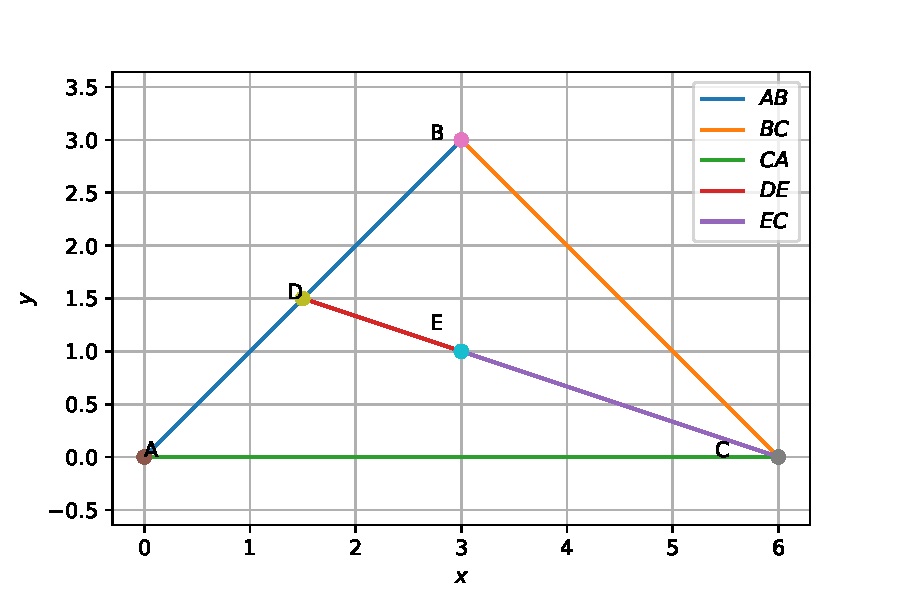
\includegraphics[width=\columnwidth]{./solutions/2/22/Ex1prob22.pdf}
    \caption{For $l=1,m=1,k=1$ and $A(0,0),B(3,3)\, $\&$\, C(6,0)$, the solution $E(3,1)$ is obtained using Python}
    \label{eq:solutions/2/22/f2}
\end{figure}
       


\end{enumerate}
